
\serie{Symétrie axiale}

\begin{exercice}[Figures symétriques ?]
Dans chaque cas, indique si les figures verte et orange sont symétriques par rapport à une droite.
\begin{center} 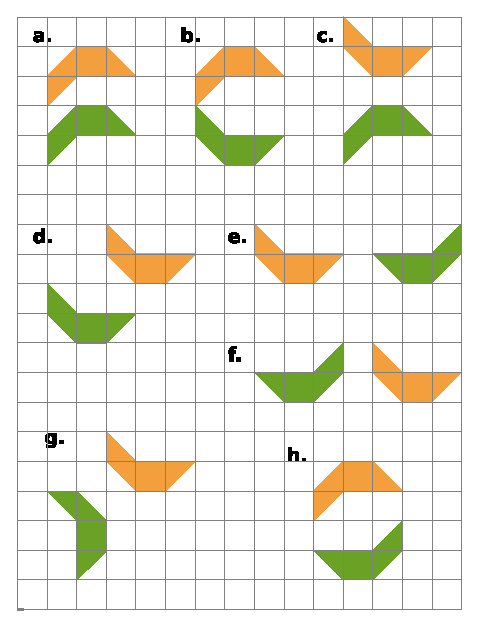
\includegraphics[width=7.9cm]{figures_sym} \end{center}
\end{exercice}


\begin{exercice}[Figures symétriques ? (bis)]
Dans chaque cas, indique si les figures mauve et bleue sont symétriques par rapport à une droite.
\begin{center} 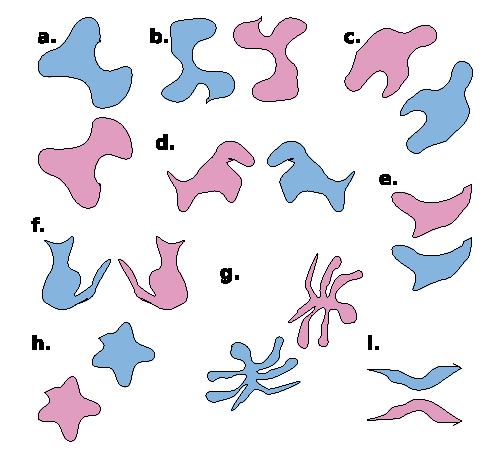
\includegraphics[width=8.1cm]{figures_sym2} \end{center}
\end{exercice}


\begin{exercice}[Erreurs à trouver]
Pourquoi les figures ocre et verte ne sont-elles pas symétriques par rapport à la droite $d$ ?
\begin{center} 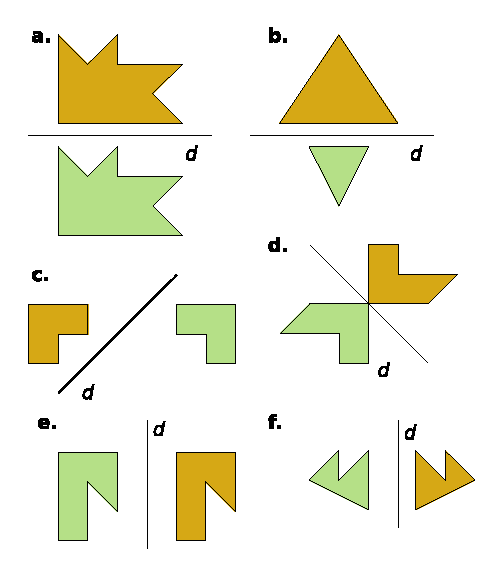
\includegraphics[width=7.9cm]{figures_erreurs} \end{center}
\end{exercice}


\begin{exercice}[Figure à plier]
\begin{minipage}[c]{0.62\linewidth}
Sur du papier calque, trace une droite rouge. Cette droite partage ton calque en deux.

Dessine un motif en t'inspirant du dessin ci‑contre sur la première moitié du calque, puis plie ton calque et complète ton dessin pour que ta figure soit symétrique par rapport à l'axe noir.
 \end{minipage} \hfill%
 \begin{minipage}[c]{0.36\linewidth}
 \begin{center} 
\includegraphics[width=1.7cm]{papillon} \end{center}
  \end{minipage} \\
\end{exercice}


\begin{exercice}[Jeu des différences]
Retrouve les erreurs qui se sont glissées sur ces deux figures pour qu'elles soient parfaitement symétriques par rapport à la droite rouge.
\begin{center} 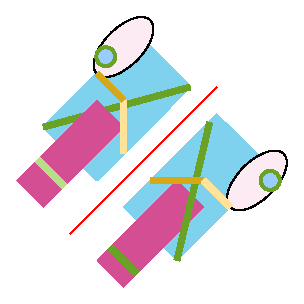
\includegraphics[width=5cm]{jeu_differences} \end{center}
\end{exercice}


\begin{exercice}[Points symétriques]
\begin{enumerate}
 \item Sur la figure ci‑dessous, cite les couples de points qui sont symétriques par rapport à l'axe rouge. \\[0.3em]
 \begin{center} 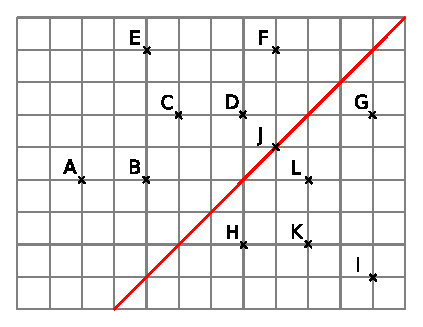
\includegraphics[width=6.9cm]{quadrillage_axerouge} \end{center}
 \item Fais trois phrases du type : « L'axe rouge est l'axe de symétrie du segment \ldots ».
 \item Reproduis cette figure et complète‑la pour que chaque point ait un symétrique.
 \end{enumerate}
\end{exercice}


\begin{exercice}[Cases croisées]
Reproduis et colorie le minimum de cases pour que l'axe rouge soit un axe de symétrie.
 \begin{center} 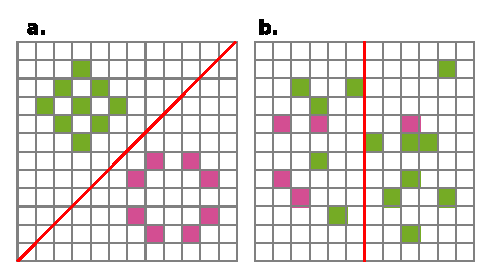
\includegraphics[width=8.1cm]{cases_croisees} \end{center}
\end{exercice}


\begin{exercice}[Frise]
Reproduis la figure ci‑dessous puis trace son symétrique par rapport à l'axe rouge. 
 \begin{center} 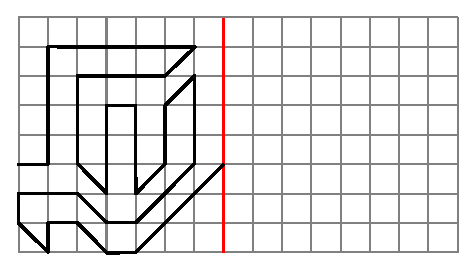
\includegraphics[width=7.9cm]{frise} \end{center}
\end{exercice}


\begin{exercice}
Reproduis puis trace le symétrique de chaque figure par rapport à $d$.

\begin{minipage}[c]{0.48\linewidth}
 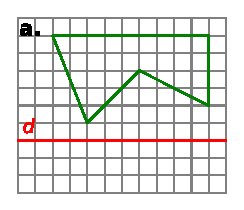
\includegraphics[width=3.7cm]{repro_d1}
 \end{minipage} \hfill%
 \begin{minipage}[c]{0.48\linewidth}
 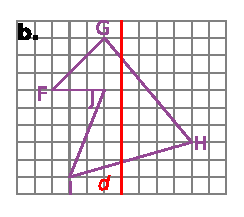
\includegraphics[width=3.7cm]{repro_d2}
  \end{minipage} \\
 \begin{minipage}[c]{0.48\linewidth}
 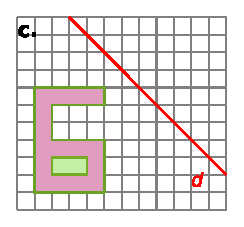
\includegraphics[width=3.7cm]{repro_d3}
 \end{minipage} \hfill%
 \begin{minipage}[c]{0.48\linewidth}
 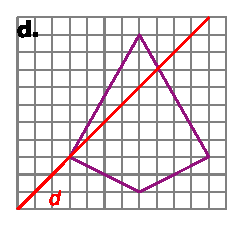
\includegraphics[width=3.7cm]{repro_d4}
 \end{minipage} \\
\end{exercice}


%%%%%%%%%%%%%%%%%%%%%%%%%%%%%%%%%%%
%%%%%%%%%%%%%%%%%%%%%%%%%%%%%%%%%%%
%MiseEnPage
%%%%%%%%%%%%%%%%%%%%%%%%%%%%%%%%%%%
\newpage
%%%%%%%%%%%%%%%%%%%%%%%%%%%%%%%%%%%
%%%%%%%%%%%%%%%%%%%%%%%%%%%%%%%%%%%

\begin{exercice}[Symétrique d'un point]
\begin{enumerate}
 \item Reproduis une figure similaire à celle ci‑dessous :
 \begin{center} 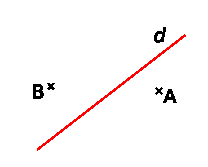
\includegraphics[width=2.8cm]{pointsABd} \end{center}
 \item Construis le symétrique par rapport à $d$ du point :
 \begin{itemize}
  \item $A$ à la règle et l'équerre ;
  \item $B$ au compas.
  \end{itemize}   
 \item Soit $H$ le point d'intersection de $(AB)$ avec $d$. Que dire de son symétrique par rapport à $d$ ?
 \end{enumerate} 
\end{exercice}


\begin{exercice}[Symétrique d'un triangle]
\begin{minipage}[c]{0.52\linewidth}
\begin{enumerate}
 \item Reproduis une figure similaire à celle ci-contre ;
 \item Construis au compas le symétrique du triangle $GHI$ par rapport à $d$.
 \end{enumerate}
 \end{minipage} \hfill%
 \begin{minipage}[c]{0.44\linewidth}
  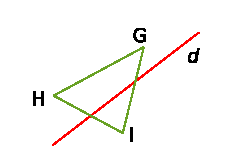
\includegraphics[width=3cm]{triangleGHId}
   \end{minipage} \\
\end{exercice}


\begin{exercice}[Symétrique d'un cercle]
\begin{enumerate}
 \item Trace un cercle $\mathcal{C}$ de centre $G$ et de rayon 5 cm. Place deux points $A$ et $B$ sur ce cercle non diamétralement opposés.
 \item Trace le symétrique de $\mathcal{C}$ par rapport à $(AB)$.
 \item Par quels points passent les deux cercles ? Justifie.
 \item Que se passe‑t‑il si $A$ et $B$ sont diamétralement opposés ?
 \end{enumerate}
\end{exercice}


\begin{exercice}[Symétrique d'une figure]
\begin{minipage}[c]{0.44\linewidth}
\begin{enumerate}
 \item Reproduis une figure similaire à celle ci‑contre ;
 \item À l'aide d'une règle et d'une équerre, trace le symétrique de cette figure par rapport à la droite $(AB)$.
 \end{enumerate}
 \end{minipage} \hfill%
 \begin{minipage}[c]{0.52\linewidth}
  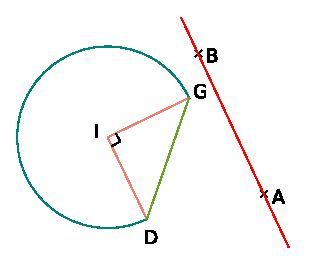
\includegraphics[width=4.5cm]{figure_droiteAB}
   \end{minipage} \\
\end{exercice}

%%%%%%%%%%%%%%%%%%%%%%%%%%%%%%%%%%%
%%%%%%%%%%%%%%%%%%%%%%%%%%%%%%%%%%%
%MiseEnPage
%%%%%%%%%%%%%%%%%%%%%%%%%%%%%%%%%%%
\columnbreak
%%%%%%%%%%%%%%%%%%%%%%%%%%%%%%%%%%%
%%%%%%%%%%%%%%%%%%%%%%%%%%%%%%%%%%%

\begin{exercice}[À propos des distances]
\begin{enumerate}
 \item Reproduis une figure similaire à celle ci‑dessous : 
 \begin{center} 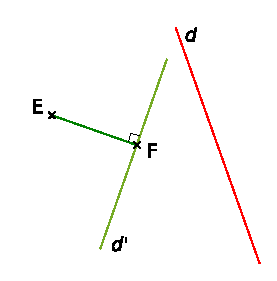
\includegraphics[width=4.7cm]{distances} \end{center}
 \item Trace le symétrique de $[EF]$ par rapport à $d$. On le note $[E'F']$. Que peux‑tu dire de la longueur de $[E'F']$ ? Justifie.
 \item Que peux‑tu dire du symétrique de $d'$ par rapport à $d$ ? Trace alors ce symétrique.
 \item Que peux‑tu dire du symétrique du cercle de diamètre $[EF]$ par rapport à $d$ ? Justifie.
 \end{enumerate}
\end{exercice}


\begin{exercice}[À propos de l'alignement]
\begin{enumerate}
 \item Trace une droite $d$. Place trois points $A$, $B$ et $C$ alignés qui n'appartiennent pas à $d$ ;
 \item Construis les points $A'$, $B'$ et $C'$ symétriques respectifs de $A$, $B$ et $C$ par rapport à $d$ ;
 \item Que dire des points $A'$, $B'$ et $C'$ ? Justifie.
 \end{enumerate}
\end{exercice}


\begin{exercice}[À propos des milieux]
\begin{enumerate}
 \item Effectue le programme de construction :
 \begin{itemize}
  \item Trace un segment $[KL]$ de longueur 7 cm ;
  \item Place le point $M$ sur $[KL]$ tel que $LM = 2$ cm ;
  \item Place le milieu $I$ de $[ML]$ ;
  \item Place le milieu $J$ de $[MK]$ ;
  \item Trace la droite $(d)$, passant par $M$ et perpendiculaire à $(KL)$ ;
  \item Trace le symétrique $I'$ de $I$ par rapport à $(d)$ et le symétrique $J'$ de $J$ par rapport à $(d)$.
  \end{itemize}
 \item Calcule, en justifiant, la longueur du segment $[I'J']$.
 \end{enumerate}
\end{exercice}

%%%%%%%%%%%%%%%%%%%%%%%%%%%%%%%%%%%
%%%%%%%%%%%%%%%%%%%%%%%%%%%%%%%%%%%
%MiseEnPage
%%%%%%%%%%%%%%%%%%%%%%%%%%%%%%%%%%%
\newpage
%%%%%%%%%%%%%%%%%%%%%%%%%%%%%%%%%%%
%%%%%%%%%%%%%%%%%%%%%%%%%%%%%%%%%%%

\begin{exercice}[À propos du périmètre]
\begin{enumerate}
 \item Trace un triangle $ABC$ tel que $AB = 5$ cm, $AC = 6$ cm et $BC = 9$ cm sur une feuille blanche.
Trace une droite $d$ parallèle à $(BC)$.
 \item Trace au compas le symétrique du triangle $ABC$ par rapport à $d$. On le note $A'B'C'$.
 \item Quel est le périmètre du triangle $A'B'C'$ ? 
 \end{enumerate}
\end{exercice}


\begin{exercice}[Sans axe]
Les deux figures ci-dessous sont symétriques par rapport à une droite.
 \begin{center} 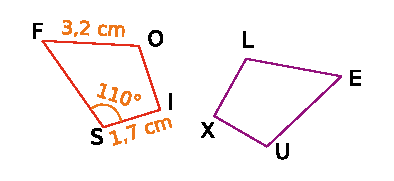
\includegraphics[width=5.9cm]{sans_axe} \end{center}
 \begin{enumerate}
 \item Reproduis et complète le tableau suivant.
 \begin{center}
  \begin{tabularx}{0.9\linewidth}{|c|*{6}{>{\centering\arraybackslash}X|}}
  \hline
\rowcolor{J1} Points & $F$ & $O$ & $I$ & $S$ \\ \hline
\rowcolor{C3} Symétriques & & & & \\ \hline
 \end{tabularx}
 \end{center}
 \vspace{0.3cm}
Tu justifieras ensuite chaque réponse.
 \item Quelle est la longueur du segment $[LE]$ ?
 \item Quelle autre longueur peux‑tu déterminer ?
 \item Quelle est la mesure de l'angle $\widehat{XUE}$ ?
 \item Écris deux autres égalités de mesure d'angles.
 \end{enumerate}
\end{exercice}


\begin{exercice}[À la recherche de l'axe]
Dans chaque cas, décalque les deux figures puis trace l'axe de symétrie. (Tu expliqueras comment tu fais sans plier le calque.)
 \begin{center} 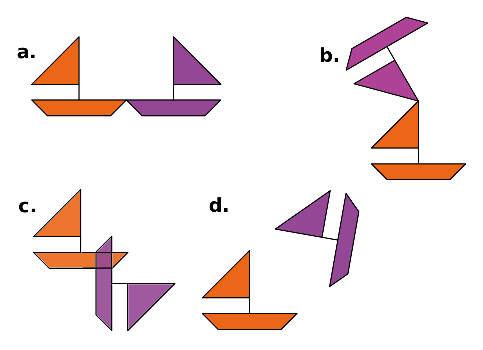
\includegraphics[width=8cm]{bateaux_colores} \end{center}
\end{exercice}

%%%%%%%%%%%%%%%%%%%%%%%%%%%%%%%%%%%%%%%%%%%%%%%%%%%%%%%%%%%%%%%%%%%%

\serie{Symétrie centrale}

\begin{exercice}
À l'aide de la règle graduée, retrouve, sur la figure ci-dessous, toutes les paires de points qui semblent symétriques par rapport au point $N$ : 
 \begin{center} 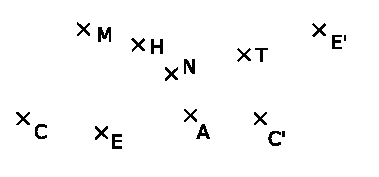
\includegraphics[width=5.8cm]{many_points} \end{center}
\end{exercice}


\begin{exercice}
Reforme des phrases correctes en associant les bonnes cases et recopie-les sur ton cahier :
\begin{center}
\renewcommand*\tabularxcolumn[1]{>{\centering\arraybackslash}m{#1}}
\begin{ttableau}{\linewidth}{3}
 \cline{1-1}\cline{3-3}
 \small{$A'$ est le symétrique du point $A$ par rapport au point $O$ donc \ldots} & & \small{$A'$ est le milieu du segment $[OA]$.} \\  \cline{1-1}\cline{3-3}
 \small{$O$ est l'image du point $A$ par la symétrie de centre $A'$ donc \ldots} & & \small{$A$ est le milieu du segment $[OA']$.} \\  \cline{1-1}\cline{3-3}
 \small{Le point $A'$ se transforme en $O$ par la symétrie de centre $A$ donc \ldots} & & \small{$O$ est le milieu du segment $[AA']$.} \\  \cline{1-1}\cline{3-3}
 \end{ttableau}
 \end{center}
\end{exercice}


\begin{exercice}
Dans chaque cas, reproduis la lettre sur du papier quadrillé et construis son symétrique par rapport au point $G$ :
 \begin{center} 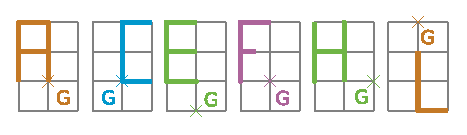
\includegraphics[width=7.7cm]{lettresG} \end{center}
\end{exercice}


\begin{exercice}
Sur ton cahier, reproduis la figure ci-dessous et construis les symétriques des points $P$, $R$ et $O$ par rapport au point $F$ :
 \begin{center} 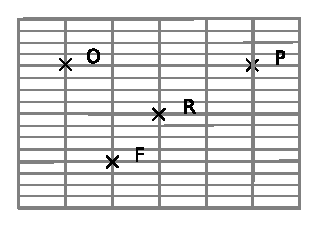
\includegraphics[width=5cm]{cahierFORP} \end{center}
\end{exercice}


\begin{exercice}
Sur ton cahier, reproduis la figure et construis le symétrique du mot MAT par rapport au point $R$ puis le symétrique du mot obtenu par rapport à la droite $d$ :
 \begin{center} 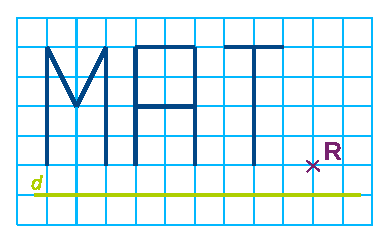
\includegraphics[width=6.3cm]{MAT} \end{center}
\end{exercice}


\begin{exercice}
Dans chaque cas, reproduis la figure et construis le point $D$, symétrique du point $A$ par rapport au point $C$ puis le point $E$, symétrique du point $C$ par rapport au point $B$ :
\begin{colenumerate}{2}
 \item 
 
 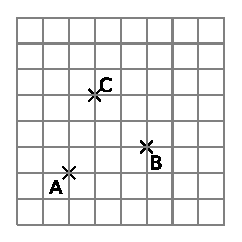
\includegraphics[width=3.7cm]{symCAB1}
 \item 
 
 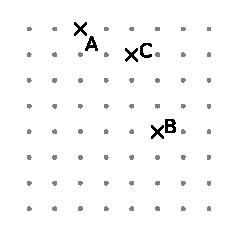
\includegraphics[width=3.7cm]{symCAB2}
 \end{colenumerate}
\end{exercice}


\begin{exercice}

\begin{minipage}[c]{0.48\linewidth}
Reproduis séparément chaque triangle sur du papier quadrillé et construis son symétrique par rapport au point $S$ :
 \end{minipage} \hfill%
 \begin{minipage}[c]{0.48\linewidth}
 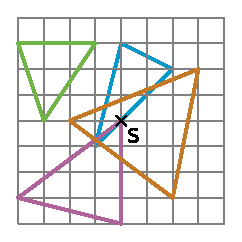
\includegraphics[width=3.7cm]{triangles_symS}
 \end{minipage} \\
\end{exercice}


\begin{exercice}
Reproduis les figures ci-dessous sur du papier quadrillé et construis le symétrique de chacune d'elles par rapport au point $H$ :
\begin{colenumerate}{2}
 \item 

 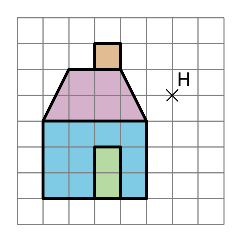
\includegraphics[width=3.7cm]{maison_sym}

 \item
 
 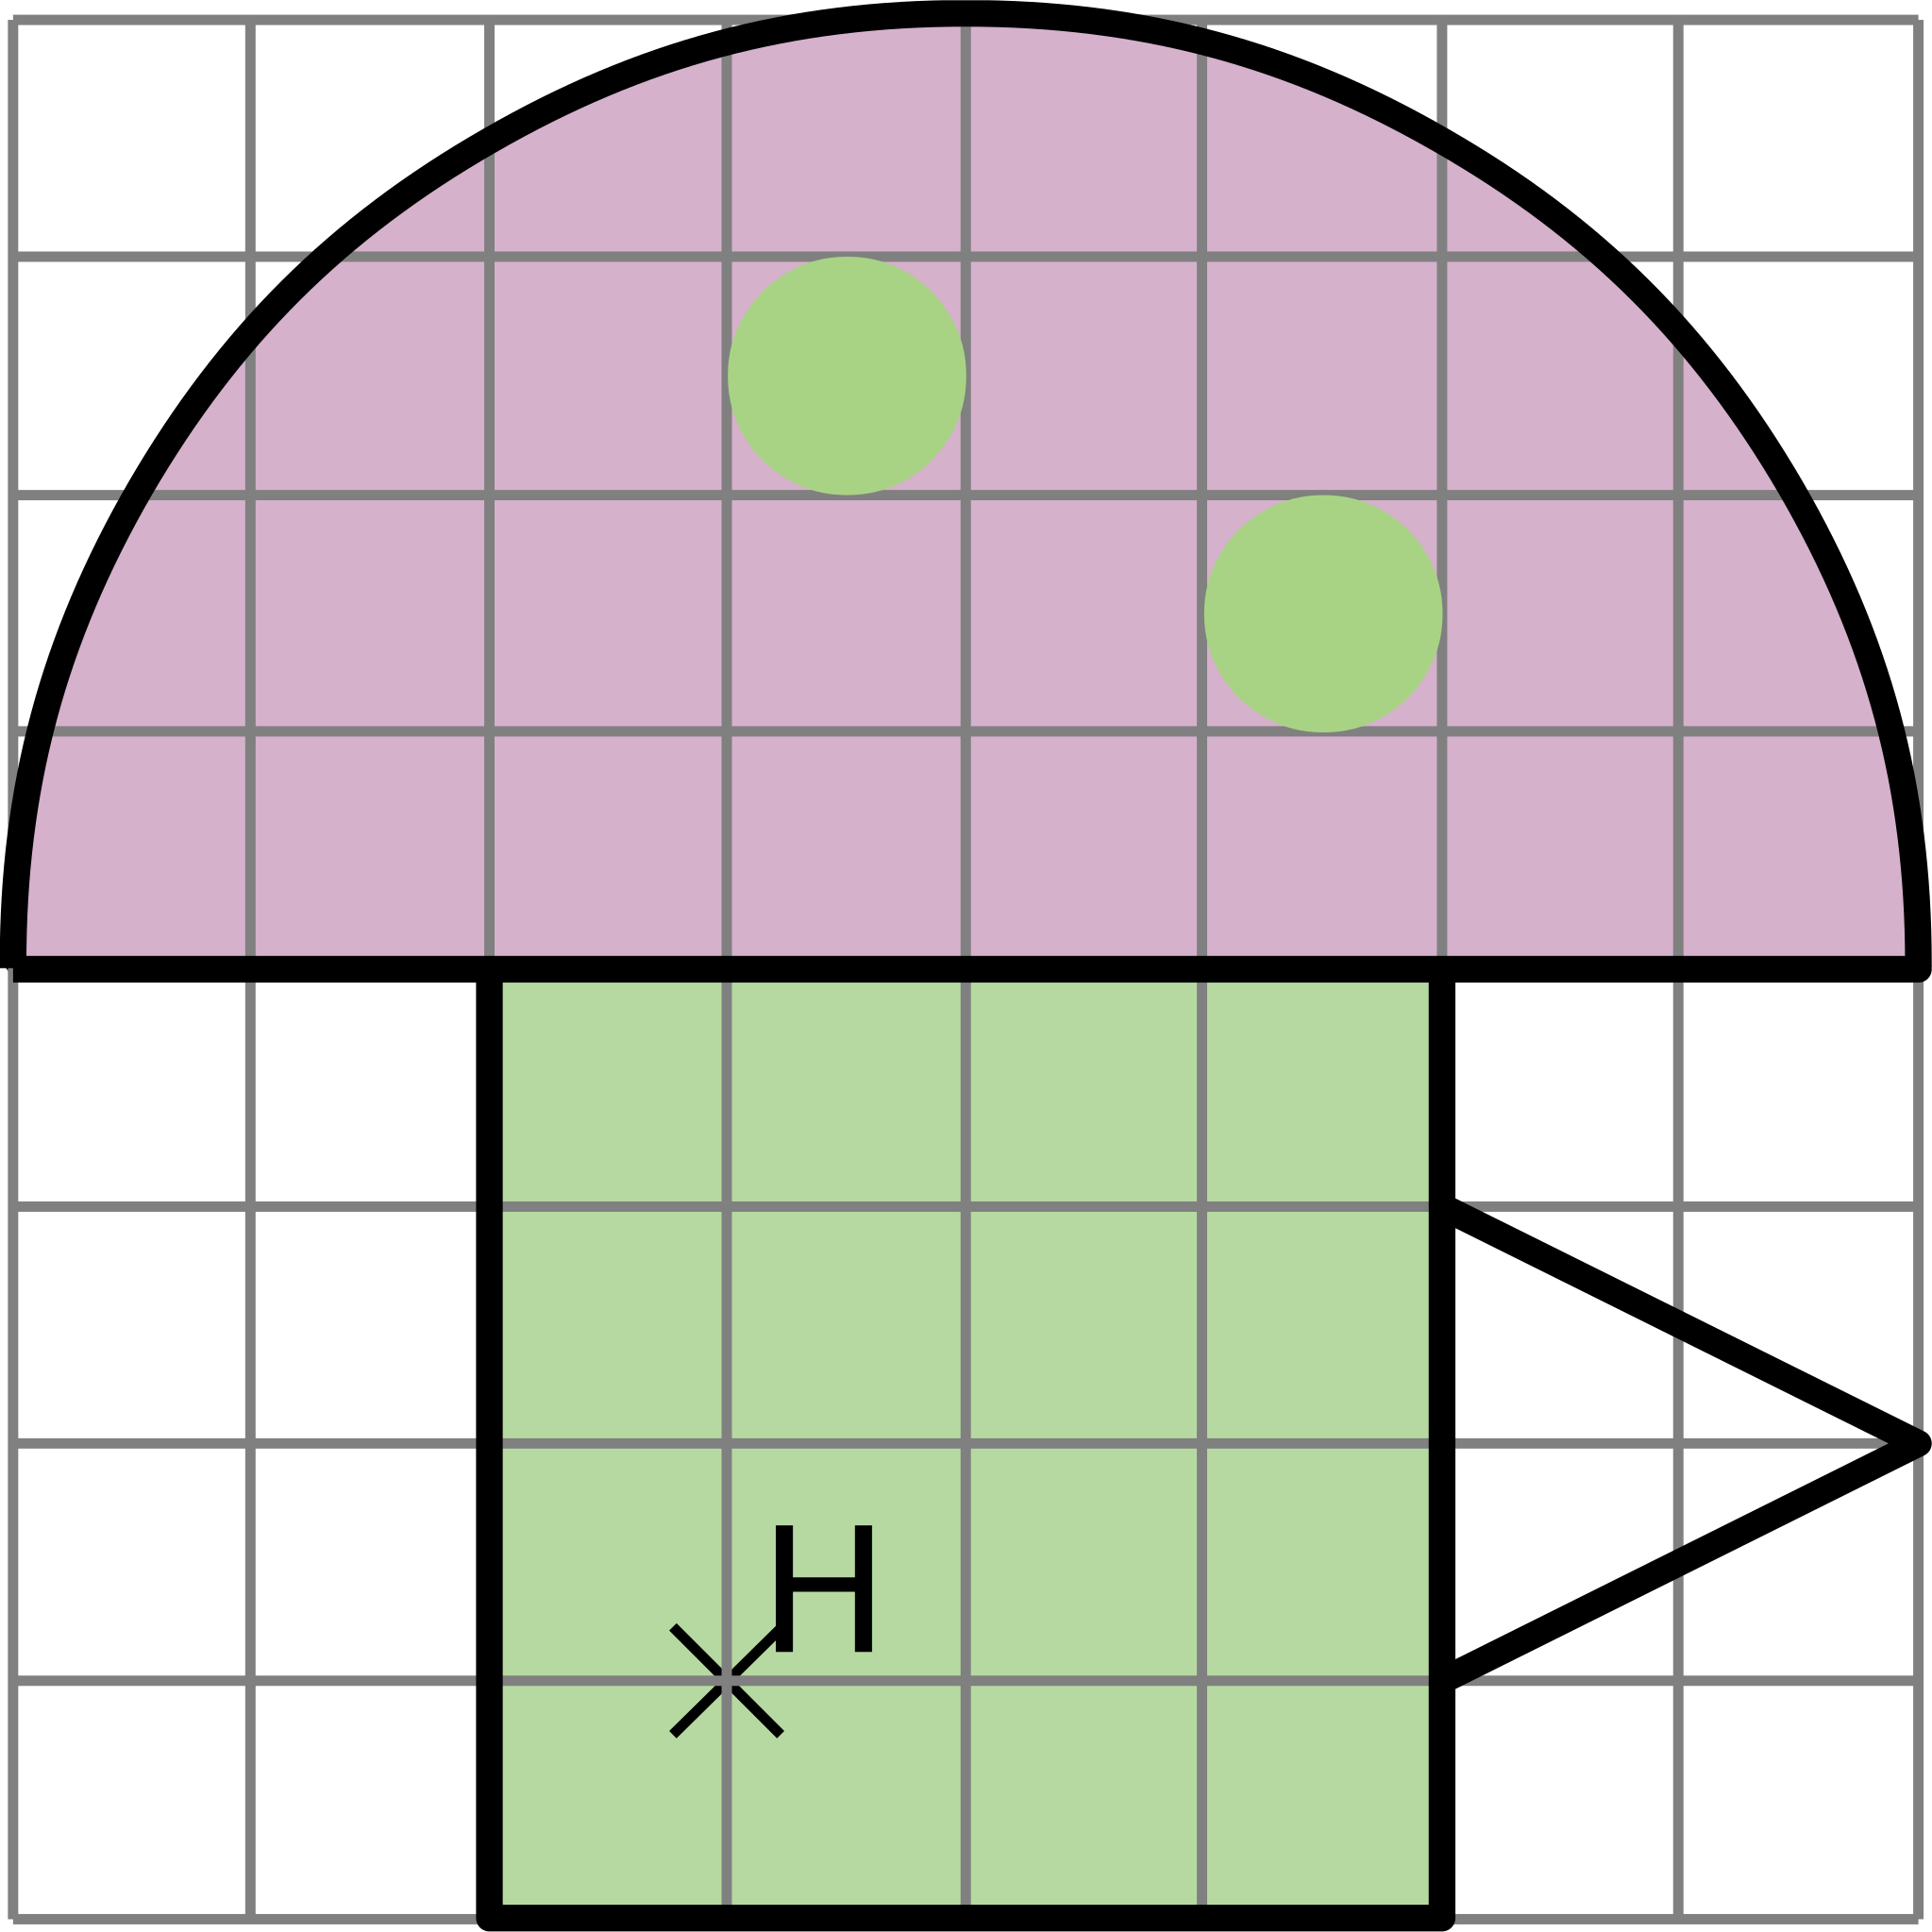
\includegraphics[width=3.7cm]{champignon_sym}
 \end{colenumerate}
\end{exercice}


\begin{exercice}

\begin{minipage}[c]{0.48\linewidth}
Sur la figure ci-contre, $ROSE$ est un carré de centre $H$. Les points $I$, $J$, $K$ et $L$ sont les milieux respectifs des côtés $[RO]$, $[OS]$, $[SE]$ et $[RE]$.
 \end{minipage} \hfill%
\begin{minipage}[c]{0.48\linewidth}
 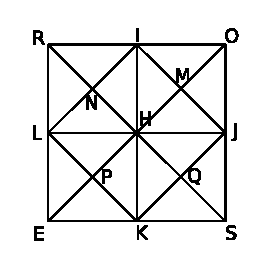
\includegraphics[width=3.7cm]{ROSE}
 \end{minipage} \\
 \begin{enumerate}
  \item Reproduis la figure en prenant $RO = 8$ cm ;
  \item Colorie en jaune le triangle $RNI$ ;
  \item Colorie en rouge le symétrique du triangle $RNI$ par rapport à la droite $(IK)$ puis en orange le symétrique du triangle $RNI$ par rapport à la droite $(LJ)$ ;
  \item Colorie en bleu le symétrique du triangle $RNI$ par rapport au point $N$ puis en vert le symétrique du triangle $RNI$ par rapport au point $H$.
 \end{enumerate}
\end{exercice}


\begin{exercice}
Dans chacun des quatre cas suivants, des élèves ont voulu tracer la figure symétrique du bateau bleu par rapport au point $C$. Les tracés sont-ils exacts ? Explique pourquoi. 
\begin{colenumerate}{2}
 \item 
 
 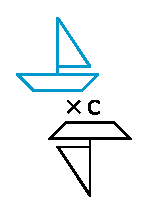
\includegraphics[width=2.3cm]{bateaux_bn1}
 \item 
 
 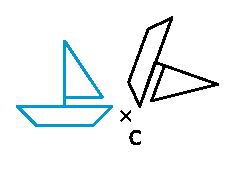
\includegraphics[width=3.7cm]{bateaux_bn2}
 \item 
 
 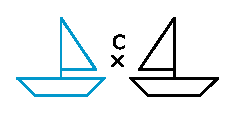
\includegraphics[width=3.7cm]{bateaux_bn3}
 \item 
 
 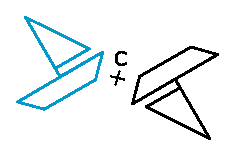
\includegraphics[width=3.7cm]{bateaux_bn4}
 \end{colenumerate}
\end{exercice}


\begin{exercice}
Place trois points $A$, $B$ et $C$ non alignés tels que $AB = 5$ cm et $AC = 3$ cm. Construis, avec seulement la règle graduée, les points $B'$ et $C'$ symétriques respectifs des points $B$ et $C$ par rapport au point $A$.
\end{exercice}


\begin{exercice}
Reproduis la figure ci-dessous et construis, avec la règle non graduée et le compas, les symétriques des points $M$ et $R$ par rapport au point $E$ :
 \begin{center} 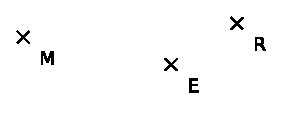
\includegraphics[width=4.4cm]{pointsMER} \end{center}
\end{exercice}


\begin{exercice}
Reproduis chaque figure et construis le symétrique du segment $[AB]$ par rapport au point $S$ :
\begin{colenumerate}{3}
 \item 
 
 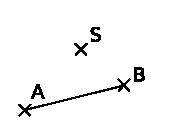
\includegraphics[width=2cm]{pointsSAB_1}
  \item 
 
 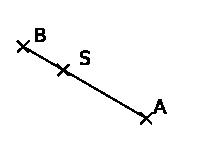
\includegraphics[width=2cm]{pointsSAB_2}
  \item 
 
 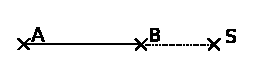
\includegraphics[width=2.5cm]{pointsSAB_3}
 \end{colenumerate}
\end{exercice}


\begin{exercice}
Reproduis chaque figure et construis le symétrique de la droite $d$ par rapport au point $U$ :
\begin{colenumerate}{2}
 \item 
 
 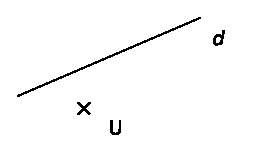
\includegraphics[width=3.5cm]{pointsUd}
  \item 
 
 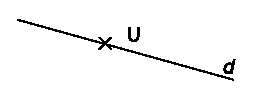
\includegraphics[width=3.5cm]{pointsUd2}
 \end{colenumerate}
\end{exercice}


\begin{exercice}
Reproduis chaque figure en prenant 5 cm pour le rayon du cercle puis construis le symétrique du cercle par rapport au point $T$ :
\begin{colenumerate}{3}
 \item 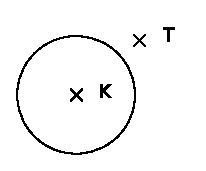
\includegraphics[width=2cm]{cercleKT1}
 \item 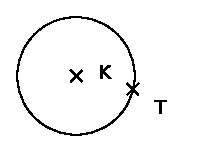
\includegraphics[width=2cm]{cercleKT2}
 \item 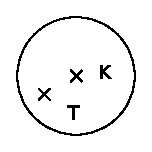
\includegraphics[width=1.4cm]{cercleKT3}
 \end{colenumerate}
\end{exercice}


\begin{exercice}
Construis un triangle $EFG$ rectangle en $E$ tel que $EF = 3$ cm et $EG = 5$ cm.
\begin{enumerate}
 \item Place le point $M$ milieu du segment $[EF]$ puis construis les points $E_1$, $F_1$ et $G_1$ symétriques respectifs des points $E$, $F$ et $G$ par rapport au point $M$ ;
 \item Construis les points $E_2$, $F_2$ et $G_2$ images respectives des points $E_1$, $F_1$ et $G_1$  par la symétrie de centre $E$ ;
 \item Place le point $K$ milieu du segment $[FG]$ puis construis les points $E_3$, $F_3$ et $G_3$ symétriques respectifs des points $E$, $F$ et $G$ par rapport au point $K$ ;
 \item Les points $E_3$, $F_3$ et $G_3$ sont les images respectives des points $E_2$, $F_2$ et $G_2$ par la symétrie de centre $O$. Quelle semble être la position de ce point $O$ ? Place-le sur ta figure.
 \end{enumerate}
\end{exercice}


\begin{exercice}[Figures complexes]
\begin{enumerate}
 \item Reproduis la figure ci-dessous, en haut à gauche avec $AB = 8$ cm et $AD = 5$ cm. Le point $E$ est le milieu du segment $[AB]$. 
 \begin{center} 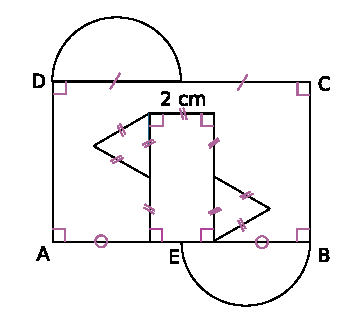
\includegraphics[width=5.2cm]{fig_complexes} \end{center}
 \item Construis le symétrique de cette figure par rapport au point $B$.
 \end{enumerate}
\end{exercice}


\begin{exercice}
Construis un rectangle $MATH$ tel que $MA = 5$ cm et $AT = 7$ cm puis place le point $E$ sur le côté $[AT]$ tel que $AE = 2$ cm. Construis en rouge le symétrique du rectangle $MATH$ par rapport au point $E$.
\end{exercice}


\begin{exercice}
Parmi les cartes ci-dessous, quelles sont celles qui possèdent un centre de symétrie ? 
 \begin{center} 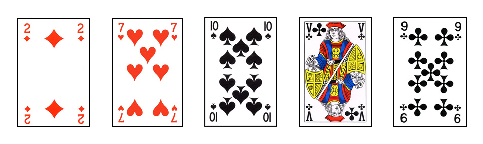
\includegraphics[width=7.7cm]{cartes_poker1} \end{center}
\end{exercice}

%%%%%%%%%%%%%%%%%%%%%%%%%%%%%%%%%%%
%%%%%%%%%%%%%%%%%%%%%%%%%%%%%%%%%%%
%MiseEnPage
%%%%%%%%%%%%%%%%%%%%%%%%%%%%%%%%%%%
\newpage
%%%%%%%%%%%%%%%%%%%%%%%%%%%%%%%%%%%
%%%%%%%%%%%%%%%%%%%%%%%%%%%%%%%%%%%

\begin{exercice}
Marine affirme que toutes les cartes ci-dessous possèdent un centre de symétrie. A-t-elle raison ? Justifie ta réponse.
 \begin{center} 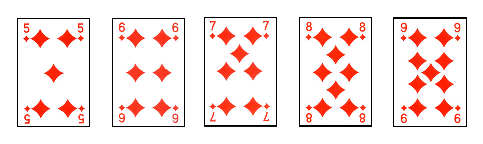
\includegraphics[width=7.7cm]{cartes_poker2} \end{center}
\end{exercice}


\begin{exercice}
Reproduis les lettres ci-dessous puis, trace en vert l'axe (ou les axes) de symétrie et en rouge le centre de symétrie de chaque lettre lorsqu'il(s) existe(nt) :
 \begin{center} 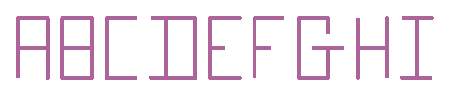
\includegraphics[width=7.4cm]{lettres_grandes} \end{center}
\end{exercice}


\begin{exercice}
Sur la figure ci-dessous, le point $B$ est le symétrique du point $A$ par rapport à $O$ :
 \begin{center} 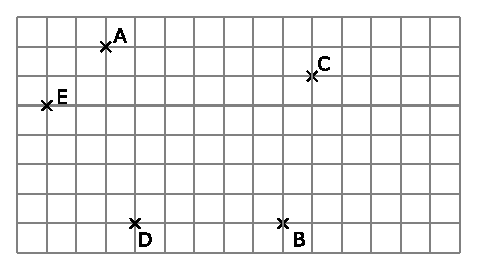
\includegraphics[width=7.9cm]{quadrillageABCDE} \end{center}
\begin{enumerate}
 \item Reproduis la figure ci-dessus puis place le point $O$ ;
 \item En t'aidant du quadrillage, place les points $C'$, $D'$ et $E'$ symétriques respectifs des points $C$, $D$ et $E$ par rapport à $O$.
 \end{enumerate}
\end{exercice}


\begin{exercice}
Reproduis puis complète la figure ci-dessous pour que $O$ soit un centre de symétrie de celle-ci :
 \begin{center} 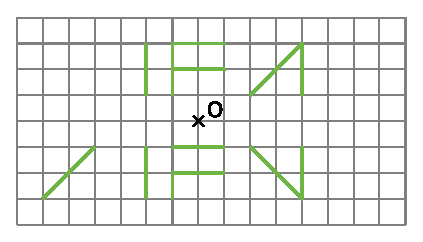
\includegraphics[width=6.9cm]{quadrillage_figsym} \end{center}
\end{exercice}


\begin{exercice}
Reproduis puis colorie le minimum de cases pour que chacune des figures ci-dessous admette le point $O$ pour centre de symétrie :

\begin{minipage}[c]{0.48\linewidth}
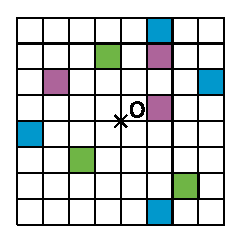
\includegraphics[width=3.7cm]{carreaux_colores1}
 \end{minipage} \hfill%
\begin{minipage}[c]{0.48\linewidth}
 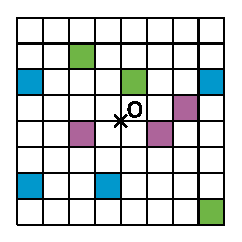
\includegraphics[width=3.7cm]{carreaux_colores2}
 \end{minipage} \\

\end{exercice}


\begin{exercice}
Reproduis la figure ci-dessous et complète-la de telle sorte que le centre du rectangle vert soit le centre de symétrie de la figure :
 \begin{center} 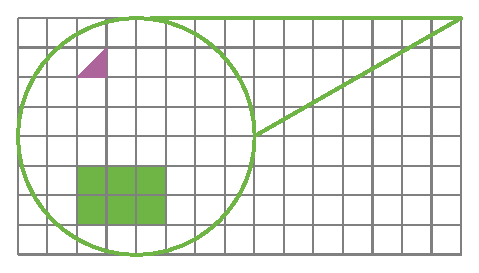
\includegraphics[width=7.9cm]{fig_completer} \end{center}
\end{exercice}


\begin{exercice}[Nombres et centre de symétrie]
Christian a écrit les chiffres comme ci-dessous :
 \begin{center} \includegraphics[width=7.7cm]{nombres_grands} \end{center}
 \begin{enumerate}
  \item Il dit : « Si je fais le double du produit de 17 par 29, j'obtiens le plus grand nombre de trois chiffres différents qui possède un centre de symétrie. ». A-t-il raison ? 
  \item Trouve le plus petit nombre de trois chiffres différents dont l'écriture possède un centre de symétrie. Écris ce nombre et place le centre de symétrie.
  \end{enumerate}
\end{exercice}


\begin{exercice}
Soit un angle $\widehat{BAD}$ mesurant $120^\circ$ tel que $AB = 4$ cm et $AD = 5$ cm. Soit $C$ un point tel que le quadrilatère non croisé formé par les points $A$, $B$, $C$ et $D$ admette un centre de symétrie.
\begin{enumerate}
 \item Trace une figure à main levée.
 \item Combien y a-t-il de positions possibles pour le point $C$ ? Pour chaque cas, indique la position du centre de symétrie.
 \item Trace autant de figures qu'il y a de centres de symétrie et indique pour chaque cas le nom et la nature du quadrilatère ainsi construit.
 \end{enumerate}
\end{exercice}


\begin{exercice}
Éric a commencé la phrase suivante :
 \begin{center} « Le symétrique par rapport à $O$ d'un triangle isocèle est ... . ». \end{center}
 \begin{enumerate}
  \item Peux-tu compléter sa phrase ?
  \item Éric a oublié de justifier sa phrase. Fais-le pour lui.
  \item Écris deux autres phrases du même type en n'oubliant pas de justifier.
  \end{enumerate}
\end{exercice}


\begin{exercice}
On a tracé, à main levée, deux figures symétriques par rapport à $O$ :
 \begin{center} \includegraphics[width=7.9cm]{polygones_sym} \end{center}
\begin{enumerate}       
 \item Indique le symétrique par rapport à $O$ de chaque sommet du polygone $ABCDE$.
 \item Donne la longueur du segment $[PK]$. Justifie ta réponse.
 \item Donne la mesure de l'angle $\widehat{NPK}$. Justifie ta réponse.
 \item De quelles autres informations disposes-tu  concernant le polygone $KLMNP$ ? Pourquoi ?
 \end{enumerate}
\end{exercice}

%%%%%%%%%%%%%%%%%%%%%%%%%%%%%%%%%%%
%%%%%%%%%%%%%%%%%%%%%%%%%%%%%%%%%%%
%MiseEnPage
%%%%%%%%%%%%%%%%%%%%%%%%%%%%%%%%%%%
\columnbreak
%%%%%%%%%%%%%%%%%%%%%%%%%%%%%%%%%%%
%%%%%%%%%%%%%%%%%%%%%%%%%%%%%%%%%%%

\begin{exercice}[Histoire d'angles]
\begin{enumerate}
 \item Construis un angle $\widehat{xOy}$ mesurant $74^\circ$ puis place un point $A$ sur $[Ox)$ et un point $B$ sur $[Oy)$ ;
 \item Construis les points $C$ et $D$ symétriques respectifs de $B$ et de $O$ par rapport à $A$ ;
 \item Sans utiliser le rapporteur, mais en justifiant les réponses, donne la mesure de l'angle $\widehat{CDA}$ et compare les mesures des angles $\widehat{BAO}$ et $\widehat{DAC}$ ;
 \item Que peut-on dire des droites $(BD)$ et $(CO)$ ? Justifie ta réponse.
 \end{enumerate}
\end{exercice}


\begin{exercice}[Symétrie et périmètre]
\begin{enumerate}
 \item Trace un triangle $ABC$, isocèle en $A$ tel que $AB = 6$ cm et $BC = 3$ cm. Place le point $I$, milieu du segment $[BC]$ ;
 \item Construis le point $D$ symétrique du point $A$ par rapport à $I$ ;
 \item Donne les longueurs $DB$ et $DC$ puis le périmètre de $ABDC$ ;
 \item Quelle est la nature du quadrilatère $ABDC$ ? Justifie ta réponse.
 \end{enumerate}
\end{exercice}


\begin{exercice}
$ABC$ est un triangle tel que $AB = 4$ cm, $AC = 5$ cm et $BC = 6$ cm. $I$ désigne le milieu de $[AB]$ et $D$ le symétrique de $C$ par rapport à $I$.
\begin{enumerate}
 \item Construis la figure.
 \item Sans mesurer, mais en justifiant tes réponses, donne les mesures AD et BD.
 \end{enumerate}
\end{exercice}
